
%%%%%%%%%%%%%%%%%%%%%%%%%%%%%%%%%%%%%%%%%%%%%%%%%%%%%%%%%%%%%%%%%%%%%%%%%%%%%%%%%%%%%%%
%%%%%%%%%%%%%%%%%%%%%%%%%%%%%%%%%%%%%%%%%%%%%%%%%%%%%%%%%%%%%%%%%%%%%%%%%%%%%%%%%%%%%%%
% 
% This top part of the document is called the 'preamble'.  Modify it with caution!
%
% The real document starts below where it says 'The main document starts here'.

\documentclass[12pt]{article}

\usepackage{amssymb,amsmath,amsthm}
\usepackage[top=1in, bottom=1in, left=1.25in, right=1.25in]{geometry}
\usepackage{fancyhdr}
\usepackage{enumerate}
\usepackage{listings}
\usepackage{graphicx}
\usepackage{float}
\usepackage{multicol}
% Comment the following line to use TeX's default font of Computer Modern.
\usepackage{times,txfonts}
\usepackage{mwe}
\usepackage{caption}
\usepackage{subcaption}

\usepackage{tikz}
\def\checkmark{\tikz\fill[scale=0.4](0,.35) -- (.25,0) -- (1,.7) -- (.25,.15) -- cycle;} 



\makeatletter
\renewcommand*\env@matrix[1][*\c@MaxMatrixCols c]{%
  \hskip -\arraycolsep
  \let\@ifnextchar\new@ifnextchar
  \array{#1}}
\makeatother

\newtheoremstyle{homework}% name of the style to be used
  {18pt}% measure of space to leave above the theorem. E.g.: 3pt
  {12pt}% measure of space to leave below the theorem. E.g.: 3pt
  {}% name of font to use in the body of the theorem
  {}% measure of space to indent
  {\bfseries}% name of head font
  {:}% punctuation between head and body
  {2ex}% space after theorem head; " " = normal interword space
  {}% Manually specify head
\theoremstyle{homework} 

% Set up an Exercise environment and a Solution label.
\newtheorem*{exercisecore}{Exercise \@currentlabel}
\newenvironment{exercise}[1]
{\def\@currentlabel{#1}\exercisecore}
{\endexercisecore}

\newcommand{\localhead}[1]{\par\smallskip\noindent\textbf{#1}\nobreak\\}%
\newcommand\solution{\localhead{Solution:}}

%%%%%%%%%%%%%%%%%%%%%%%%%%%%%%%%%%%%%%%%%%%%%%%%%%%%%%%%%%%%%%%%%%%%%%%%
%
% Stuff for getting the name/document date/title across the header
\makeatletter
\RequirePackage{fancyhdr}
\pagestyle{fancy}
\fancyfoot[C]{\ifnum \value{page} > 1\relax\thepage\fi}
\fancyhead[L]{\ifx\@doclabel\@empty\else\@doclabel\fi}
\fancyhead[C]{\ifx\@docdate\@empty\else\@docdate\fi}
\fancyhead[R]{\ifx\@docauthor\@empty\else\@docauthor\fi}
\headheight 15pt

\def\doclabel#1{\gdef\@doclabel{#1}}
\doclabel{Use {\tt\textbackslash doclabel\{MY LABEL\}}.}
\def\docdate#1{\gdef\@docdate{#1}}
\docdate{Use {\tt\textbackslash docdate\{MY DATE\}}.}
\def\docauthor#1{\gdef\@docauthor{#1}}
\docauthor{Use {\tt\textbackslash docauthor\{MY NAME\}}.}
\makeatother

% Shortcuts for blackboard bold number sets (reals, integers, etc.)
\newcommand{\Reals}{\ensuremath{\mathbb R}}
\newcommand{\Nats}{\ensuremath{\mathbb N}}
\newcommand{\Ints}{\ensuremath{\mathbb Z}}
\newcommand{\Rats}{\ensuremath{\mathbb Q}}
\newcommand{\Cplx}{\ensuremath{\mathbb C}}
%% Some equivalents that some people may prefer.
\let\RR\Reals
\let\NN\Nats
\let\II\Ints
\let\CC\Cplx

%\textbf{Code:}
%\begin{center}
%  \lstinputlisting{NewtonsMethodP5.m}
%\end{center}
%
%\textbf{Console:}
%\begin{center}
%  \lstinputlisting{P5C.txt}
%\end{center}
%\vspace{.15in}


%\begin{figure}[H]
%  \begin{center}
%    \caption{The one-norm unit ball}
%    \includegraphics[width=.76\textwidth]{1norm.png}
%  \end{center}
%\end{figure}




%%%%%%%%%%%%%%%%%%%%%%%%%%%%%%%%%%%%%%%%%%%%%%%%%%%%%%%%%%%%%%%%%%%%%%%%%%%%%%%%%%%%%%%
%%%%%%%%%%%%%%%%%%%%%%%%%%%%%%%%%%%%%%%%%%%%%%%%%%%%%%%%%%%%%%%%%%%%%%%%%%%%%%%%%%%%%%%
% 
% The main document start here.

% The following commands set up the material that appears in the header.
\doclabel{Math 661: Project Proposal}
\docauthor{Stefano Fochesatto}
\docdate{\today}
%As an aside I will be using 
%graph theory terms from now on, and for the rest of the project, like most things in optimization it seems like 
%there exists a culture that has decided to brandish new terminology for things that are already relatively well known.

\begin{document}
My project will be mainly about Network Simplex and if there is time I'd like to explore the 
applications in semantic image segmentation. As an introduction I'll describe one of the main 
network optimization problems, namely the \emph{minimum cost network flow problem}.  
Suppose you have a directed graph (network) where each vertex is assigned a value called flow and the weights on 
the edges represent the cost of moving one unit of flow. Consider the example below, 

\begin{figure}[H]
  \begin{center}
    \caption{Graph $G = \{E, V\}$ with flow $b$ and weights $c$}
    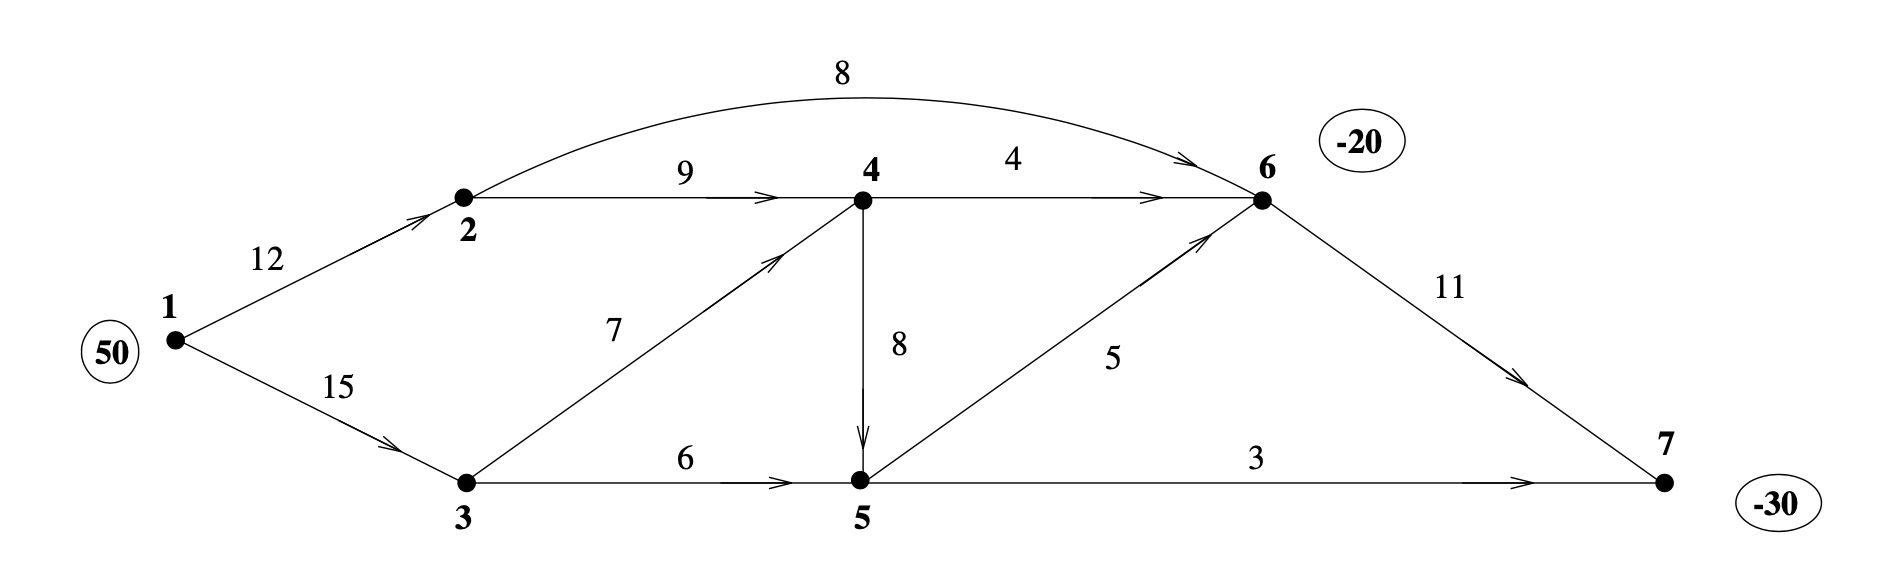
\includegraphics[width=.90\textwidth]{SampleNetwork.png}
  \end{center}
\end{figure}
If a vertex has positive flow we call it a source, and if vertex has negative flow we call it a sink. 
We define Supply, $S$ as 
\begin{equation*}
  S = \sum_{b_i > 0\in b}b_i,
\end{equation*}
and Demand, $D$ as
\begin{equation*}
  D = \sum_{b_i < 0 \in b}b_i.
\end{equation*}
We call a network balanced if $S - D = 0$, and an unbalanced network can be made balanced by adding an artificial vertex with flow $S - D$ by a directed edge with 
zero cost. The goal of the minimum cost network flow problem is to satisfy the supply and demand of each vertex while minimizing the cost. The objective function will look 
like this, 
\begin{equation*}
  \text{min } z = c^Tx
\end{equation*}
where $x_{i,j} \in x$ represents the amount of flow through edge $(i, j)$. A feasible solution to this problem is an $x$ that satisfies the supply and demand of each vertex. 
With that context at each vertex $i$ our $x$ must satisfy, 
\begin{equation*}
  \sum_{j}x_{i, j} - \sum_{k}x_{k, i} = b_i.
\end{equation*} 
One can think of the first sum being flow out of vertex $i$ and the second sum being flow into vertex $i$. As an example consider vertex $1$ and $2$ in Figure 1, 
we get the following constraints
\begin{equation*}
  x_{1, 2} + x_{1,3} = 50,
\end{equation*}
\begin{equation*}
  x_{2, 4} + x_{2, 6} - x_{1, 2} = 0.
\end{equation*}
This is done for each vertex $i$, generating our constraint matrix $A$ which will be size (\# of vertices)$ \times $(\# of edges). Usually there will be some added constraints $L$ and $U$ on the amount of flow that can go through each edge, so most problems will be of the form, 
\begin{align*}
  \text{minimize } z = c^Tx\\
  Ax = b\\
  L \leq x \leq U
\end{align*}
Since $A$ is a matrix full of either $1, 0$ or $-1$ and is usually relatively sparse with $b$ also being a sparse vector, the possibility of degeneracy (where $x_b$ in Simplex becomes zero)
is common if this LP problem is handed to a general LP solver. Network Simplex modifies the Simplex algorithm to take advantage of the idea that a feasible solution to this problem represents a 
spanning tree, resulting in a considerable speed up\cite{grivanashsofer}(8.4) and resolves common degeneracy and stalling issues by using graph analog of perturbation method\cite{grivanashsofer}(8.5). \\


Following the discussion of Network Simplex, I would like to discuss duality in the context of network algorithms. The \emph{maximum flow problem} which involves
finding the maximum flow that can be transmitted between two vertices (a single source and sink), is equivalent to a special form of the minimum cost network flow problem\cite{grivanashsofer}(p.278). The dual of this problem is the \emph{minimum cut problem}, which finds the set of edges which must be removed from a graph
to separate two vertices into disconnected subgraphs, while minimizing the weight of the removed edges (one of those 'A famous theorem states' in our textbook).  \\


This then would lead to the application in semantic image segmentation as a form of the minimum cut problem. In this context we need to be able to turn 
an image into a graph, whose edges are appropriately weighted so that solution to the minimum cut problem generates a good segmentation. The following image\cite{image} attempts to describe the this graph is generated, 
\begin{figure}[H]
  \begin{center}
    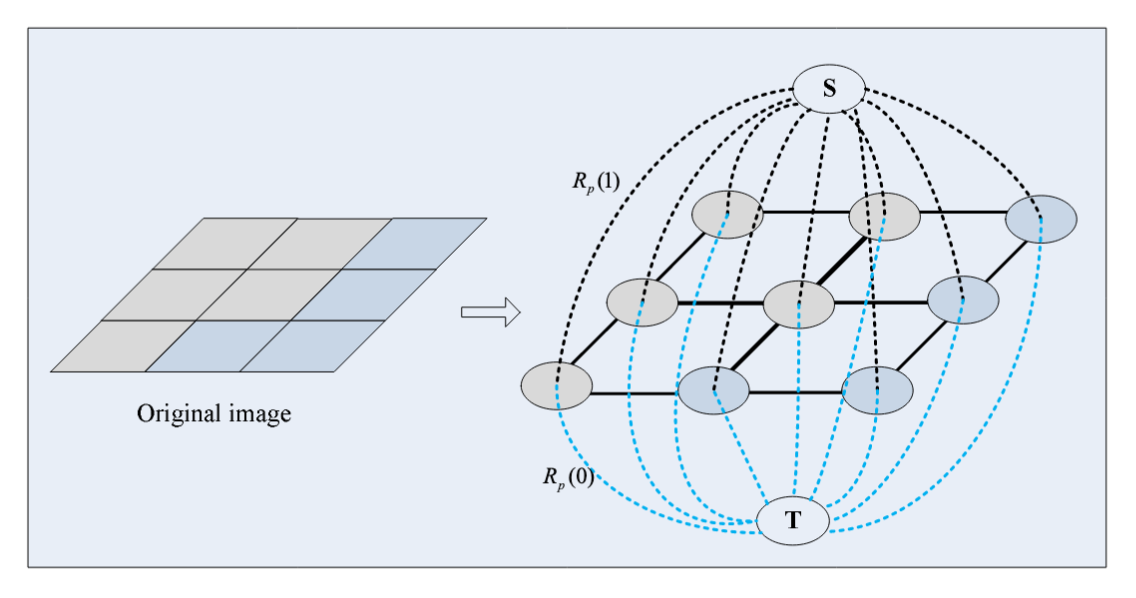
\includegraphics[width=.70\textwidth]{Image.png}
  \end{center}
\end{figure}
A user is meant to supply a seed (source and sink pixels $s$ and $t$), the weights are determined by some similarity function between pixels and the minimum cut problem is solved. 


\begin{thebibliography}{2}  % "2" because there are two references

  \bibitem{grivanashsofer}
  I.~Griva, S.~Nash, \& A.~Sofer (2009).
  \textit{Linear and Nonlinear Optimization},
  2nd ed., SIAM Press.

  \bibitem{image}
  Yi, F., \& Moon, I. (2012). 
  Image segmentation: A survey of graph-cut methods. 2012 International Conference on Systems and Informatics (ICSAI2012), 1936–1941. https://doi.org/10.1109/ICSAI.2012.6223428

  \end{thebibliography}
\end{document}


















Senning, J.R., n.d. COMPUTING AND ESTIMATING THE RATE OF CONVERGENCE 3.










